\documentclass[../Head/Main.tex]{subfiles}
\begin{document}
\section{Counting Pumpkins}\label{sec:counting}
Receiving the segmented and filtered image as described in section \ref{sec:seg}, the task was now counting the pumpkins. Two considered approaches are described in this section. To evaluate the methods qualitatively, found pumpkins are marked with circles in the original image. This method is utilized throughout this section. Furthermore, information regarding the GSD is here described. The code used for section \ref{subsec:algorithms} and \ref{subsec:gsd} is countained in files \url{src/ex3_5.py} and \url{src/ex6.py}, respectively.

\subsection{Counting Algorithms}\label{subsec:algorithms}
First, the contours were found on the filtered image using openCV's contour detection method. The center point of each contour is extracted and the resulting information along with the original openCV contour is stored in a class \verb+Contours+ found in file \url{src/contours.py}. The found contours were marked with the above mentioned method. The resulting image is seen in figure \ref{fig:contours}.

\begin{figure}[H]
\centering
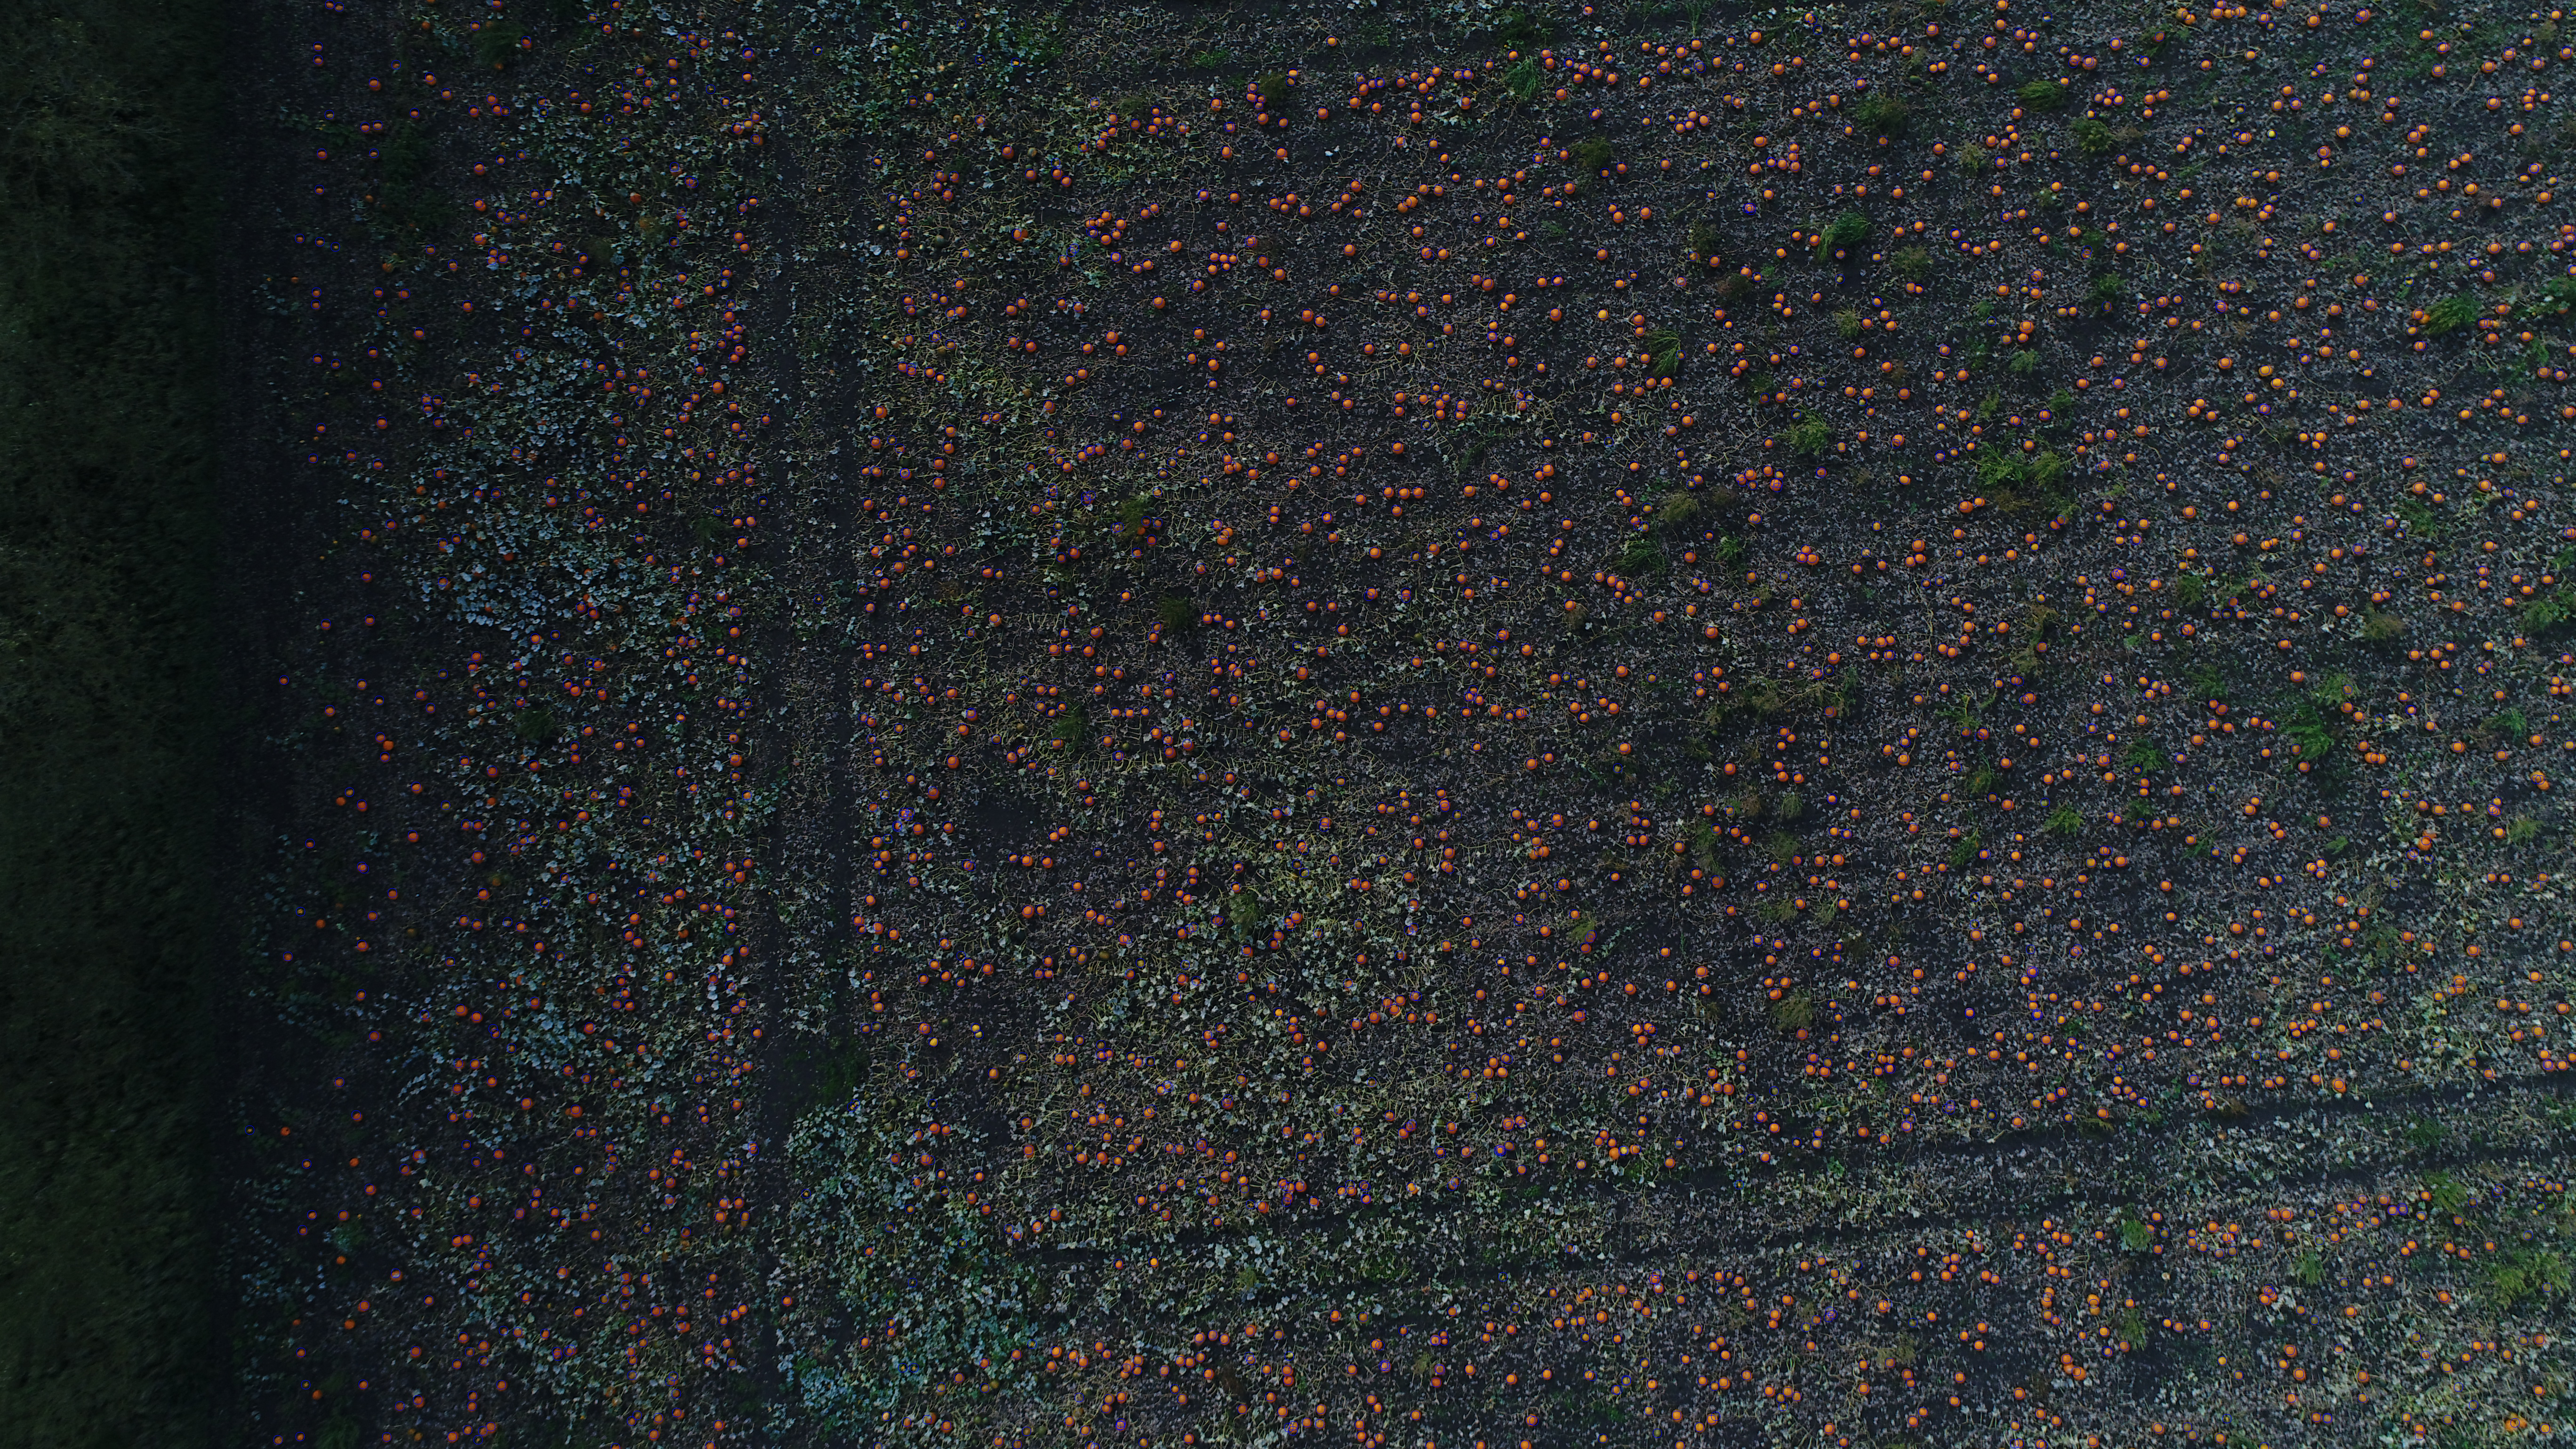
\includegraphics[width=0.8\textwidth]{../Figures/ex3_5_marked_contours_all.png}
\caption{All found contours marked}
\label{fig:contours}
\end{figure}

As can be seen, in some places several contours are found for the same pumpkin yielding too many overlapping contours. An algorithm is needed to sort the contours.

\subsubsection{Sorting Contours by Diameter}
The simplest implemented method simply sorts the contours by diameter. A pumpkin diameter is approximated to be 20 pixels using visual inspection. A loop is implemented that only counts a contour if a contour has not already been counted that has a center point closer than one pumpkin diameter to the said contour. The code is shown below:
\begin{verbatim}
counted_pumpkins = []

    for cnt in tqdm(contours):
        is_unique = True
        for ccnt in counted_pumpkins:
            if (cnt.distance_to(ccnt) < pumpkin_diameter):
                is_unique = False
                break

        if is_unique:
            counted_pumpkins.append(cnt)
            img = cv2.circle(
                img, 
                tuple(cnt.center), 
                int(pumpkin_diameter / 2), 
                (255, 0, 0), 
                1
            )

    return len(counted_pumpkins), img
\end{verbatim}
An image of the marked counted pumpkins is seen in figure \ref{fig:pumpkinsSimple}.

\begin{figure}[H]
\centering
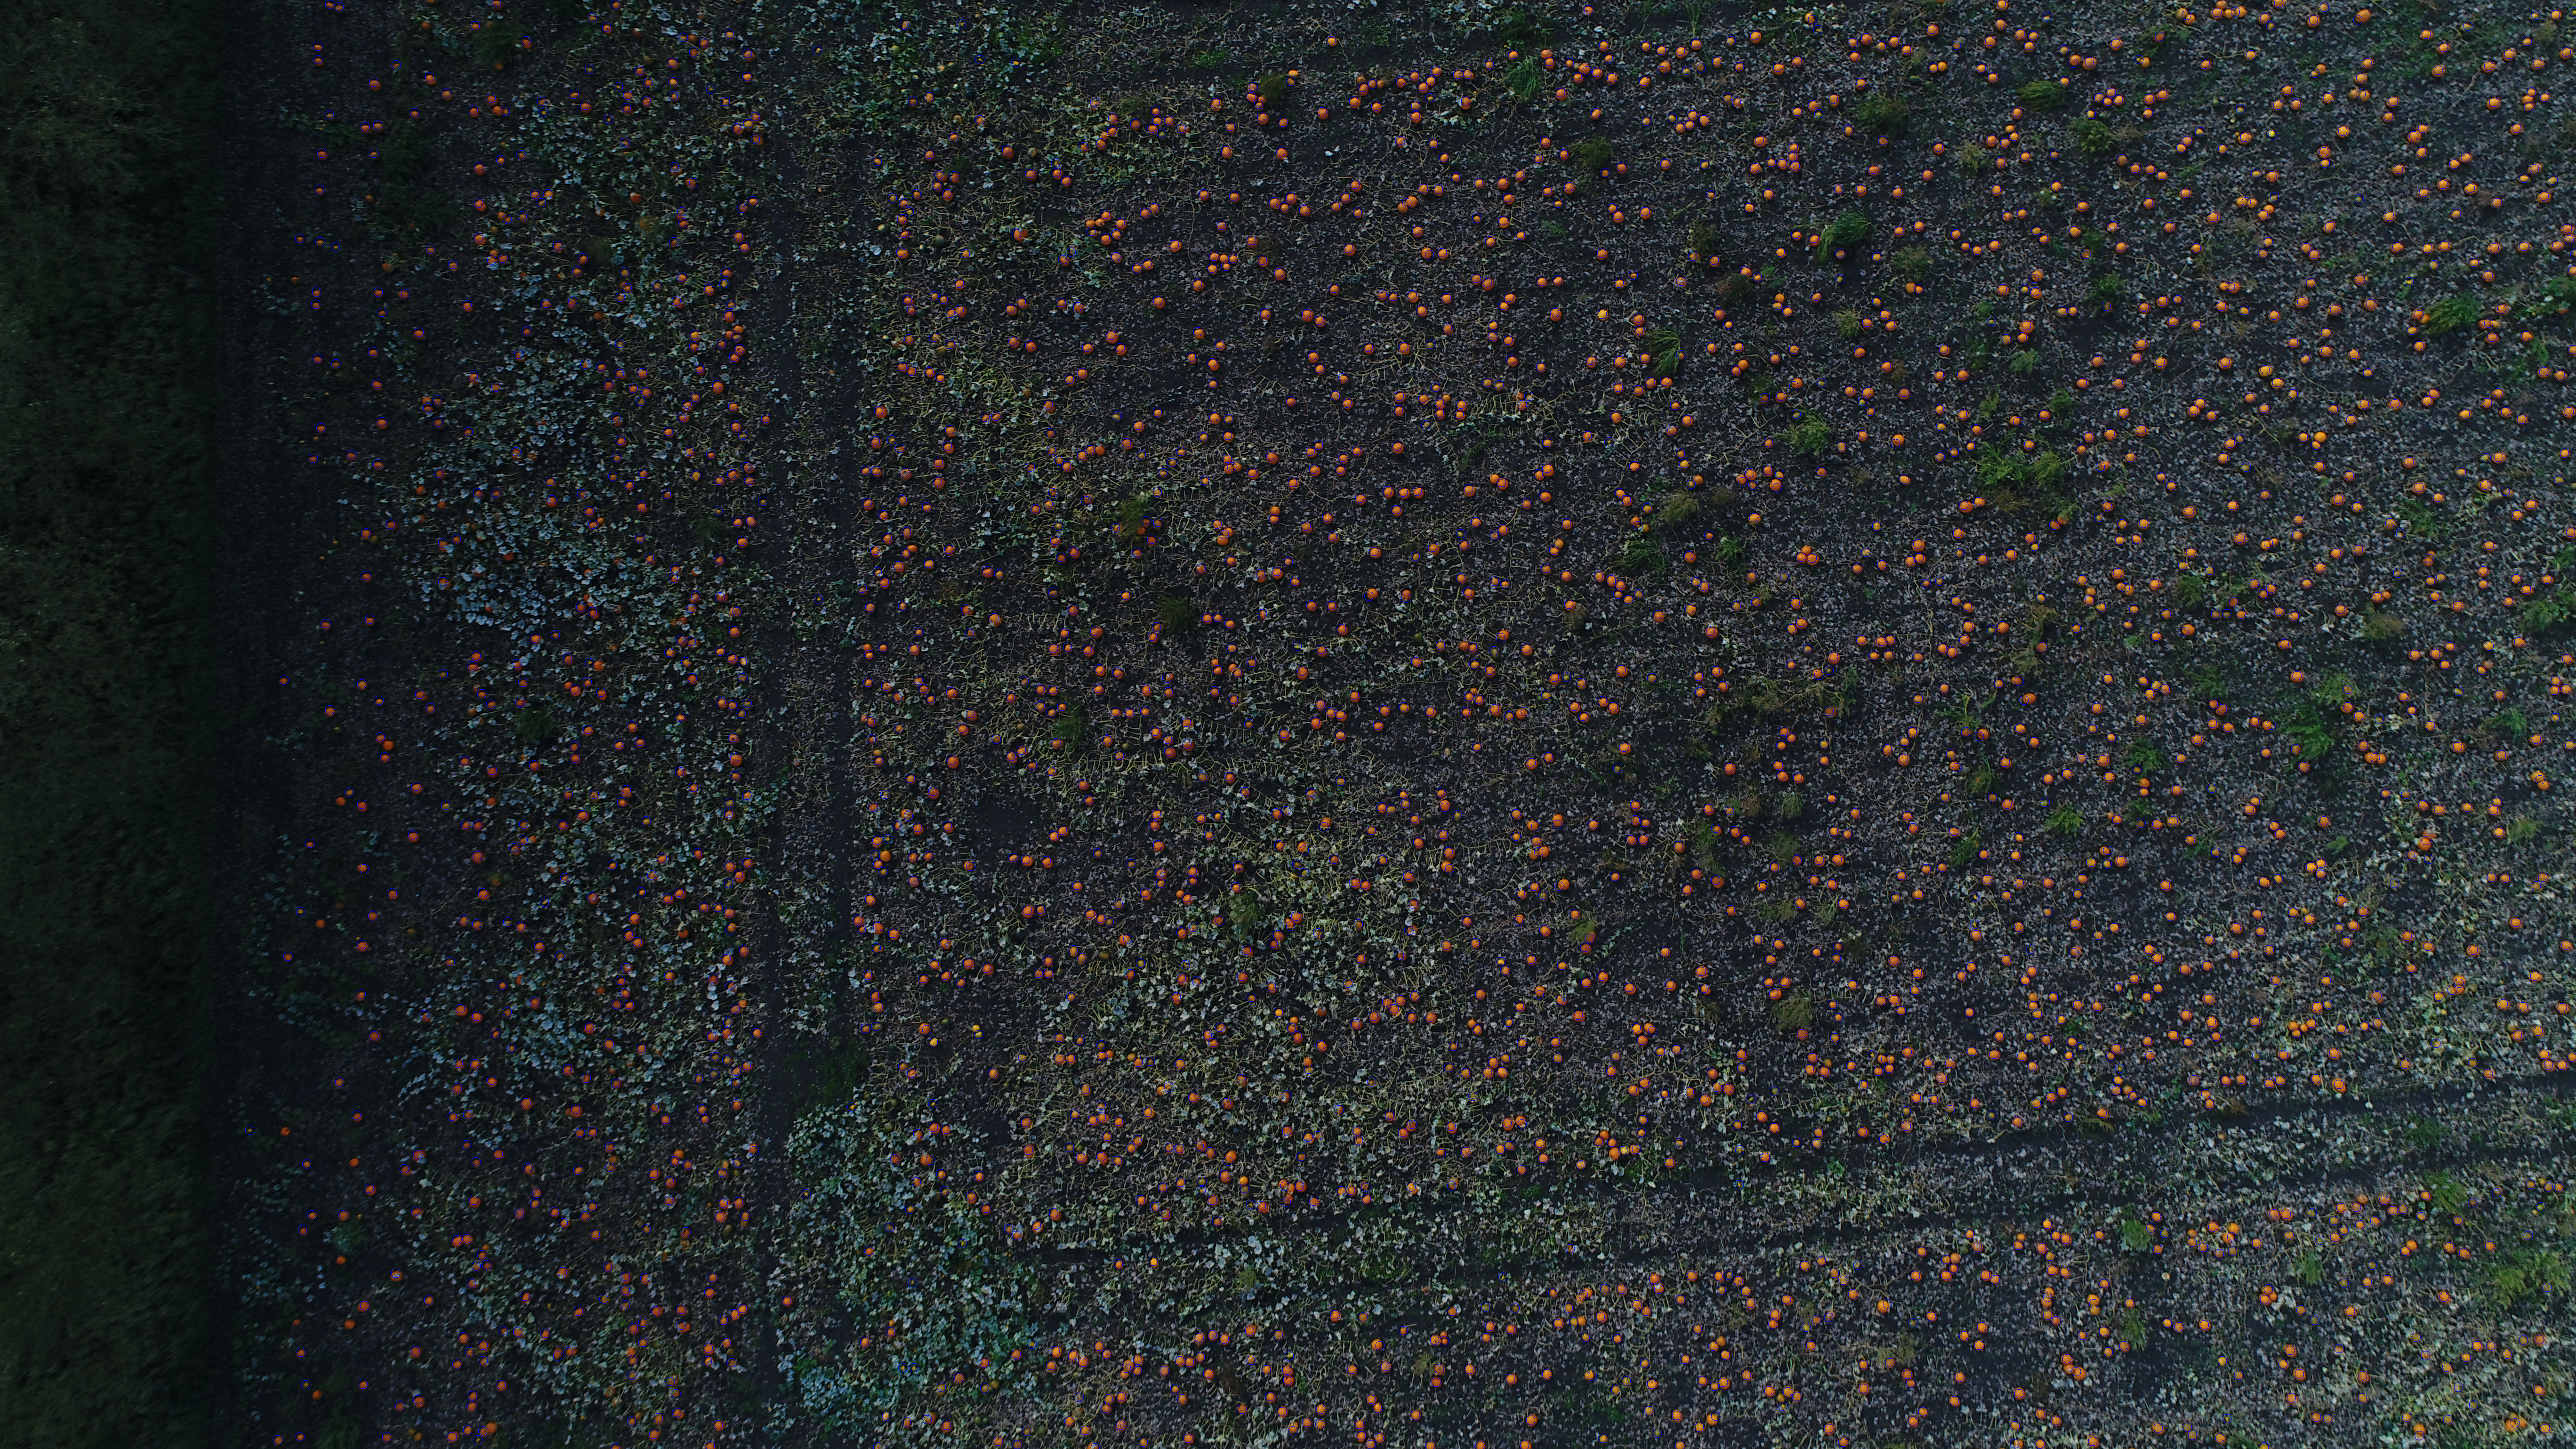
\includegraphics[width=0.8\textwidth]{../Figures/ex3_5_marked_pumpkins_simple.png}
\caption{Marked pumpkins found by the simple method.}
\label{fig:pumpkinsSimple}
\end{figure}

As can be seen, the pumpkins are counted much more correctly than before applying the algorithm. Although the system performs somewhat satisfactory, now the system is prone to missing pumpkins. This might be because the order of counting the pumpkins is more or less arbitrary. If two pumpkins are marked three times total, if the first counted contour is the middle one, the two remaining contours might not be included yielding the two pumpkins only being counted as one. 

\subsubsection{Sorting Contours with Clustering}
The hypothesis were that by clustering the obtained contours so that the distance from a contour to its nearest neighbor in the same cluster is maximum the diameter of a pumpkin, the number of pumpkins within a cluster could be estimated by inspecting the average distance for a contour to its nearest neighbor within a cluster. Theoretically, if the said average distance is 0 (or approximately 0), the number of actual pumpkins covered by the contours will be one. Likewise, if the said average distance is equal to a pumpkin diameter, the number of pumpkins covered by the contours is most likely equal to the number of contours in the cluster. As this said average distance would be maximum one pumpkin diameter, as this is the maximum allowed distance within a cluster, the said average distance can be normalized and will thus provide a scalar value to determine the number of contained pumpkins going between 1 pumpkin for average minimum distance 0 and the number of pumpkins equal to the number of contours in the cluster for the average minimum distance equal to a pumpkin diameter.\\
A class \verb+ContourCluster+ is implemented in file \url{


We used openCV's contour detector functions to find closed contours.
This leaves us with many overlapping results.

We need to find a criteria or a method to filter the undesirable matches. A simple method we tried was to use the average pumpkin diameter and disregard those mathes that have a distance to a unique match less than the average diameter.

INSERT IMAGE HERE

This method disregards a lot of real matches, and also leaves some false double matches on large targets.

The next method we tried is clustering based on a hierarchical search. The algorithm stops when the shortest distance between two clusters is more than the usual pumpkin diameter. Resulst can be seen on

INSERT IMAGE HERE

DRAW CONCLUSION ABOUT DIFFERENCES BETWEEN THE TWO METHODS

The segmentation is not that accurate on the original image. The cause of this inaccuracy can be random noise or even occluding objects like weeds or bugs. To correct for this error, we used the filter from the previous exercise and analysed the performance difference.

INSERT IMAGE HERE

DRAW CONCLUSION HERE

\subsection{GSD}\label{subsec:gsd}

If we try to measure a size on an image, the unit will be in pixels. That is not very useful if we want to get information of pumpkin sizes or number of pumpkins per square meter. To connect image units to physical units, we calculate a GSD ratio in mm/pixel.

The following source code was used for this task:

\begin{lstlisting}[language=Python]
    pixels = img.shape
    alpha = math.radians(fov_deg / 2)
    width = height_meters * 2 * math.tan(alpha)
    ratio = width / pixels[0]
    height = ratio * pixels[1]
    ratio *= 1000 # convert to mm/pixel
\end{lstlisting}

These were our parameters:

\begin{verbatim}
    Relative height: 54.2 m
    Field-of-View: 73.7 °
\end{verbatim}


We got the following results:

\begin{verbatim}
    Image width: 81.24119485997007 m
    Image height: 45.69817210873316 m
    Ratio: 14.846709586982833 mm/pixel
\end{verbatim}

\end{document}